\section{Further considerations}\label{sec:further-considerations}
    Up till now, we looked at automating the decision on what artefacts to delete first. However, efficient CI pipeline artefact storage and the related decision-making processes go beyond just the deletion of pipelines. On the following pages, we will be looking at a few related topics that could help optimise artefact retention using different methods.
    
    \subsection{Optimising retention period}
        The first related issue to tackle is storage relevancy. While we treated all pipeline artefacts as one entity in the previous experiments, this is far from the truth. In reality, each pipeline produces a large number of log files.
        
        \colfig{image/graphs/pipeline-file-count-histogram}{Pipeline file count distribution}{fig:file-count-histogram}
        
        Figure \ref{fig:file-count-histogram} depicts data extracted from a small sample of 445 pipelines from the same snapshot data set used for the size approximation in section \ref{sec:data-source-sizes}. It shows a histogram of the file counts for all observed pipelines with a bucket width of 5.000 files on the X-Axis and the percentage of all observed pipelines falling into the bucket on the Y-Axis. It should be noted that this data is not corrected for singularities like partially deleted pipelines and compressed artefacts due to the computational and storage requirements. That is likely the cause for the first bucket being filled the most. Regardless, almost 20\% of the pipeline directories contain around 80.000 to 85.000 files. We can assume that one developer is unlikely to consult all files in a given debugging session. To confirm this point, we can consult the data set we previously extracted from the simulation database to build table \ref{tbl:access-groups}. In this data, the top 10 accessed resource paths for test reports within a pipeline\footnote{Note that all paths have been stripped of unique identifies and are relative to the pipeline artifact root directory.} account for 99,2\% (8402/8471) of all requests to test reports. Similarly, the top 10 log file paths account for 60,5\% (242 out of 400). When abstracting the data further by, e.g. grouping all HTML based reports, similar results can be achieved with the top 3 paths\footnote{The raw data is confidential. See section \ref{sec:data-availability} for more detail.}. This shows that developers are mostly in need of only a handful of resources. Additionally, the most frequently accessed resources are expected to occupy only a small amount space (HTML, JSON, and XML test reports).
        
        This discovery leads to a potential hybrid or multi-stage approach. In prior experiments, pipelines were deleted once they got flagged. Given that many pipelines occupy a significant amount of storage (see figure \ref{fig:pipeline-size-histogram}), this makes sense. However, by using the information introduced in the previous paragraph, we can defer the deletion of the most frequently accessed but small files. These files would then form a second pool which could either be treated the same as the regular one or managed independently using a separate set of algorithms. Doing so would allow pipelines which would otherwise be deleted to serve at least some percentage of requests still while saving potentially multiple gigabytes of storage. It should be noted that the frequency with which a file is accessed may not be used to determine its importance. In a scenario where a very specialised log file is created with no use in day-to-day debugging operations but is crucial during a particular error condition, it would be fatal to assume it is unimportant and discard it. For that reason, this multi-stage approach should not be considered as a means to saving storage but rather as a "last chance" for a pipeline artefact on disk to be useful before being purged by partially purging it first.
        
        Another idea that could be coupled with the hybrid approach would involve the transformation of the original artefacts. An example could look like this: During the first stage, a log file contains all log levels. As disk pressure increases, messages with lower log levels are being discarded until the whole log file is deleted. This would still allow some degree of debugging instead of completely purging the file in the first place. While this approach may not satisfy all debugging scenarios, it is expected that at least under some circumstances the remaining data after a partial purge is still useful and sufficient — effectively increasing the storage density and information relevancy of the stored artefacts.

    \subsection{Increasing storage density}
        So far, we have looked at methods to increase the information density and relevancy of the data we store. However, the topic of on-disk storage density has been left untouched so far. The heatmap in figure \ref{fig:size-heatmap} shows a direct inverse relation between available disk space and access miss ratio for all algorithms observed. Based on that, we can assume that increasing the storage size yields better results. However, instead of increasing the disk size, the goal is to make better use of the disk space available. In the following two subsections, we will take a look at two methods to achieve this goal.
        
        \subsubsection{Block size}
            In order to improve performance, files are written to a physical disk in blocks. These blocks always have the same size, defined by the file-system in use and fully transparent to applications. When a file size does not align with a block boundary, it is padded with undefined data to fill the block. This space is unusable by other files. \cite{block-size-loss}
            
            When looking at figure \ref{fig:file-count-histogram} from the previous section, it becomes clear that a considerable amount of pipelines stores a large number of individual files. To approximate the lost storage due to block alignment, we will assume a block size of 4KB\footnote{This assumption is based on the recommendation by A. S. Tanenbaum et al. \cite{common-block-size}} and assert that we lose half a block on average. We may then use equation \ref{eq:block-size-loss} to get a rough estimate with a block size $b_{size}$, file count $c_{files}$, and "lost" storage amount of $s_{lost}$. In our example, we will use the high peak from the previously mentioned figure at 82.500 files.
            
            \begin{equation}\label{eq:block-size-loss}
                \begin{split}
                    s_{lost} & = \frac{b_{size}}{2} * c_{files}\\
                    s_{lost} & = \SI{2}{\kilo\byte} * 82500\\
                    s_{lost} & = \SI{165}{\mega\byte}
                \end{split}
            \end{equation}
            
            This shows that storing just over 80.000 files accounts for a storage loss of over \SI{150}{\mega\byte}. It is noteworthy that this issue is especially prevailing when using tiny files. Storing a file with just a few bytes is still going to consume at least one block. Unfortunately, we do not know the average pipeline size for the pipelines that have approximately 80.000 files.
            
            To get a closer insight into the magnitude of the issue, we will be looking at a sample pipeline extracted from the project we used for our simulation inputs instead. At first, enumerating all files and their real sizes is required. It should be noted that particular caution is required as some tools may report the size on disk instead of the file content size. The example pipeline has a total size of \SI{33}{\giga\byte} and 99,95\% of all files have a size below \SI{10}{\mega\byte}. However, the more interesting metric is how the files align with block borders. To observe this, each file size in the list has been taken modulo the block size and plotted in a histogram in figure \ref{fig:block-alignment-histogram} with a bucket width of 50 bytes. Files with a size of zero have been excluded as some file systems are known to not assign blocks to them \cite{empty-inode}.
            
            \colfig{image/graphs/block-alignment-histogram}{Block alignment losses}{fig:block-alignment-histogram}
            
            Overall, a large fraction of files have a padding of less than \SI{2}{\kilo\byte}. The median of the data set is located at 1260 bytes. It is noteworthy that many of files require around 1700 bytes of padding — the reason for this is unknown\footnote{It is likely that some files are always logged in the same format and with very similar content. However, that is just a theory based on contextual knowledge.}. In total, \SI{836}{\mega\byte} are being lost to block padding. This accounts for approximately 2,5\% of the storage used by the artefact. While this in and of itself is not a significant amount, it should still be considered part of the puzzle, and since it is highly dependent on the data at hand, the real impact might be higher.
            
            A potential solution to this issue would be to store the files in a sequential block of disk storage. This can be achieved by either concatenating all files and creating an out-of-band index elsewhere or using a standard streaming container format like \code{tar} that stores file metadata in-band. Both serve the purpose of storing files in a continuous slice of memory. Since the pipeline as a whole is now considered a single file, there is only a single block boundary which might require padding at the very end of the container.
            
            However, it should be noted that streaming container formats may not be ideal for the purpose. The \code{tar} format statically allocates 512 bytes of metadata for each file (which would cost $82500 * \SI{512}{\byte} = \SI{42,24}{\mega\byte}$ of storage), potentially nullifying the benefits\footnote{It does not in this case but is possible in general.}. Another issue with this format is the streaming focused design. As metadata is stored inline in front of each file, no central archive is available and accessing a file requires a full iteration of the archive until a matching section is found. This could be avoided by storing all files' content without metadata in one slice and having a separate out-of-band metadata block that may use additional optimisation methods to allow for fast querying of file locations within the container. However, drafting a design specification for such an archive is considered out-of-scope.\\
            \\
            When combining this archive approach with the previously outlined multi-stage approach, additional considerations need to be taken. As they are the same for the next optimisation method, we will postpone this discussion until further down the line.
            
        \subsubsection{Compression}
            Another, potentially more obvious, choice to increase the storage density is to utilise compression algorithms.
            
            \begin{Figure}
                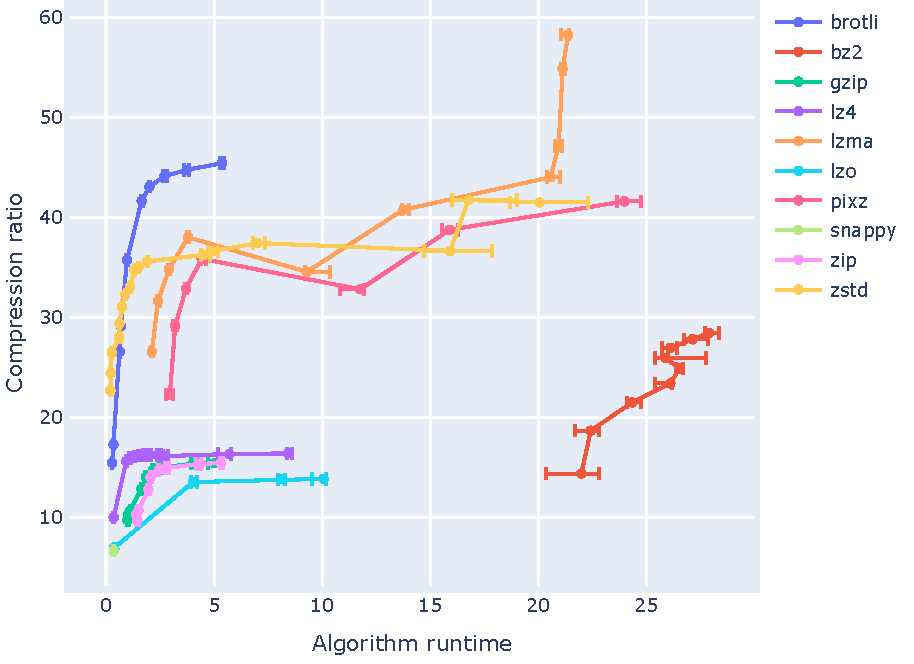
\includegraphics[width=\linewidth]{image/imported/lineplot-runtime-compressionratio}
                \captionof{figure}[Compression algorithm efficiency]{Compression algorithm efficiency \cite{tfl}}
                \label{fig:import-tfl-compressionratio}
            \end{Figure}
            
            By compressing the pipeline artefacts, a significant size reduction may be achieved. Based on the tests in a related research paper, whose main results are shown in figure \ref{fig:import-tfl-compressionratio}, a size reduction of 35 to 40 times can be achieved in a reasonable time. Allocating more compression resources allows for compression ratios as high as 58. \cite{tfl}
            
            However, compression comes with the problem of accessing the resources. Most compression formats do not allow for random access to compressed resources \cite{random-access-compression}. Based on the previously mentioned paper's research, it has become viable to retain random access capabilities while maintaining a sufficiently high size reduction using a block-based approach. With this method, the data will be split into equally sized blocks which will then be compressed individually and independently. While it is possible to maintain out-of-band metadata to improve the compression ratio theoretically, this turned out to be mostly ineffective with the given test data. \cite{tfl}
            
            It should be noted that compression algorithms are highly dependent on the input data, and thus caution should be taken when directly comparing results \cite{compression-input-dependence}. Since the research paper in question has been using the same data set as we used previously, it can be considered relevant and accurate for our use-case.
            
            Another potential hurdle to consider is the cost of rewriting a compressed pipeline. In a general sense, pipeline artefacts can be considered write-once and read-only. However, especially when using the previously mentioned multi-stage approach, some data needs to be removed, altered, or aggregated. This becomes more difficult when using any archive/container (compressed or uncompressed) as it is stored as a continuous slice of memory. Thus at least parts of the file have to be rewritten for copied. Layering compression on top compounds the problem as data may only be read/written in chunks of a fixed size, requiring additional effort at bordering chunks. Despite these potential roadblocks, it may very well still be beneficial to compress files. As the previously outlined multi-stage approach aims to retain only a small subset of the data, rewriting is expected to be reasonably fast. Since a given pipeline will only ever be written to twice during its lifetime in storage (once in the very beginning and another time when being "stripped"), the system as a whole may still be considered read-focused, and the additional cost for rewriting is very likely offset by the gains of compression.
            
            After all, this may be considered a trade-off between storage usage and CPU resources. Development operation engineers from the team observed earlier reported frequent issues with high I/O wait times\footnote{According to personal feedback these were not caused due to read speed issues but rather frequent seeks and random accesses to file-system metadata and content.} due to the file-system load with millions of files on disk. This I/O bottleneck may potentially be circumvented by offloading some work onto the CPU with either uncompressed or compressed archives — depending on the requirements.

    % \todo{Maybe this is the place for the "Static data analysis" discussion with the access times, merge times etc.}
